
%% bare_conf.tex
%% V1.4b
%% 2015/08/26
%% by Michael Shell
%% See:
%% http://www.michaelshell.org/
%% for current contact information.
%%
%% This is a skeleton file demonstrating the use of IEEEtran.cls
%% (requires IEEEtran.cls version 1.8b or later) with an IEEE
%% conference paper.
%%
%% Support sites:
%% http://www.michaelshell.org/tex/ieeetran/
%% http://www.ctan.org/pkg/ieeetran
%% and
%% http://www.ieee.org/

%%*************************************************************************
%% Legal Notice:
%% This code is offered as-is without any warranty either expressed or
%% implied; without even the implied warranty of MERCHANTABILITY or
%% FITNESS FOR A PARTICULAR PURPOSE! 
%% User assumes all risk.
%% In no event shall the IEEE or any contributor to this code be liable for
%% any damages or losses, including, but not limited to, incidental,
%% consequential, or any other damages, resulting from the use or misuse
%% of any information contained here.
%%
%% All comments are the opinions of their respective authors and are not
%% necessarily endorsed by the IEEE.
%%
%% This work is distributed under the LaTeX Project Public License (LPPL)
%% ( http://www.latex-project.org/ ) version 1.3, and may be freely used,
%% distributed and modified. A copy of the LPPL, version 1.3, is included
%% in the base LaTeX documentation of all distributions of LaTeX released
%% 2003/12/01 or later.
%% Retain all contribution notices and credits.
%% ** Modified files should be clearly indicated as such, including  **
%% ** renaming them and changing author support contact information. **
%%*************************************************************************

% *** Authors should verify (and, if needed, correct) their LaTeX system  ***
% *** with the testflow diagnostic prior to trusting their LaTeX platform ***
% *** with production work. The IEEE's font choices and paper sizes can   ***
% *** trigger bugs that do not appear when using other class files.       ***                          ***
% The testflow support page is at:
% http://www.michaelshell.org/tex/testflow/


\documentclass[conference]{IEEEtran}
% Some Computer Society conferences also require the compsoc mode option,
% but others use the standard conference format.
%
% If IEEEtran.cls has not been installed into the LaTeX system files,
% manually specify the path to it like:
% \documentclass[conference]{../sty/IEEEtran}





% Some very useful LaTeX packages include:
% (uncomment the ones you want to load)


% *** MISC UTILITY PACKAGES ***
%
%\usepackage{ifpdf}
% Heiko Oberdiek's ifpdf.sty is very useful if you need conditional
% compilation based on whether the output is pdf or dvi.
% usage:
% \ifpdf
%   % pdf code
% \else
%   % dvi code
% \fi
% The latest version of ifpdf.sty can be obtained from:
% http://www.ctan.org/pkg/ifpdf
% Also, note that IEEEtran.cls V1.7 and later provides a builtin
% \ifCLASSINFOpdf conditional that works the same way.
% When switching from latex to pdflatex and vice-versa, the compiler may
% have to be run twice to clear warning/error messages.






% *** CITATION PACKAGES ***
%
%\usepackage{cite}
% cite.sty was written by Donald Arseneau
% V1.6 and later of IEEEtran pre-defines the format of the cite.sty package
% \cite{} output to follow that of the IEEE. Loading the cite package will
% result in citation numbers being automatically sorted and properly
% "compressed/ranged". e.g., [1], [9], [2], [7], [5], [6] without using
% cite.sty will become [1], [2], [5]--[7], [9] using cite.sty. cite.sty's
% \cite will automatically add leading space, if needed. Use cite.sty's
% noadjust option (cite.sty V3.8 and later) if you want to turn this off
% such as if a citation ever needs to be enclosed in parenthesis.
% cite.sty is already installed on most LaTeX systems. Be sure and use
% version 5.0 (2009-03-20) and later if using hyperref.sty.
% The latest version can be obtained at:
% http://www.ctan.org/pkg/cite
% The documentation is contained in the cite.sty file itself.






% *** GRAPHICS RELATED PACKAGES ***
%
\ifCLASSINFOpdf
  \usepackage[pdftex]{graphicx}
  % declare the path(s) where your graphic files are
  % \graphicspath{{../pdf/}{../jpeg/}}
  % and their extensions so you won't have to specify these with
  % every instance of \includegraphics
  % \DeclareGraphicsExtensions{.pdf,.jpeg,.png}
\else
  % or other class option (dvipsone, dvipdf, if not using dvips). graphicx
  % will default to the driver specified in the system graphics.cfg if no
  % driver is specified.
  \usepackage[dvips]{graphicx}
  % declare the path(s) where your graphic files are
  % \graphicspath{{../eps/}}
  % and their extensions so you won't have to specify these with
  % every instance of \includegraphics
  % \DeclareGraphicsExtensions{.eps}
\fi
% graphicx was written by David Carlisle and Sebastian Rahtz. It is
% required if you want graphics, photos, etc. graphicx.sty is already
% installed on most LaTeX systems. The latest version and documentation
% can be obtained at: 
% http://www.ctan.org/pkg/graphicx
% Another good source of documentation is "Using Imported Graphics in
% LaTeX2e" by Keith Reckdahl which can be found at:
% http://www.ctan.org/pkg/epslatex
%
% latex, and pdflatex in dvi mode, support graphics in encapsulated
% postscript (.eps) format. pdflatex in pdf mode supports graphics
% in .pdf, .jpeg, .png and .mps (metapost) formats. Users should ensure
% that all non-photo figures use a vector format (.eps, .pdf, .mps) and
% not a bitmapped formats (.jpeg, .png). The IEEE frowns on bitmapped formats
% which can result in "jaggedy"/blurry rendering of lines and letters as
% well as large increases in file sizes.
%
% You can find documentation about the pdfTeX application at:
% http://www.tug.org/applications/pdftex





% *** MATH PACKAGES ***
%
\usepackage{bm}

\usepackage[fleqn]{amsmath}
\usepackage[psamsfonts]{amssymb}
\usepackage{url}


\newcommand{\birth}[1]{\mathcal{C}(#1)}
\newcommand{\distinct}[1]{\mathcal{N}_n^d(#1)}
\newcommand{\distinctnnn}[1]{\mathcal{N}_3^d(#1)}


%\usepackage{amsmath}
% A popular package from the American Mathematical Society that provides
% many useful and powerful commands for dealing with mathematics.
%
% Note that the amsmath package sets \interdisplaylinepenalty to 10000
% thus preventing page breaks from occurring within multiline equations. Use:
%\interdisplaylinepenalty=2500
% after loading amsmath to restore such page breaks as IEEEtran.cls normally
% does. amsmath.sty is already installed on most LaTeX systems. The latest
% version and documentation can be obtained at:
% http://www.ctan.org/pkg/amsmath





% *** SPECIALIZED LIST PACKAGES ***
%
%\usepackage{algorithmic}
% algorithmic.sty was written by Peter Williams and Rogerio Brito.
% This package provides an algorithmic environment fo describing algorithms.
% You can use the algorithmic environment in-text or within a figure
% environment to provide for a floating algorithm. Do NOT use the algorithm
% floating environment provided by algorithm.sty (by the same authors) or
% algorithm2e.sty (by Christophe Fiorio) as the IEEE does not use dedicated
% algorithm float types and packages that provide these will not provide
% correct IEEE style captions. The latest version and documentation of
% algorithmic.sty can be obtained at:
% http://www.ctan.org/pkg/algorithms
% Also of interest may be the (relatively newer and more customizable)
% algorithmicx.sty package by Szasz Janos:
% http://www.ctan.org/pkg/algorithmicx




% *** ALIGNMENT PACKAGES ***
%
%\usepackage{array}
% Frank Mittelbach's and David Carlisle's array.sty patches and improves
% the standard LaTeX2e array and tabular environments to provide better
% appearance and additional user controls. As the default LaTeX2e table
% generation code is lacking to the point of almost being broken with
% respect to the quality of the end results, all users are strongly
% advised to use an enhanced (at the very least that provided by array.sty)
% set of table tools. array.sty is already installed on most systems. The
% latest version and documentation can be obtained at:
% http://www.ctan.org/pkg/array


% IEEEtran contains the IEEEeqnarray family of commands that can be used to
% generate multiline equations as well as matrices, tables, etc., of high
% quality.




% *** SUBFIGURE PACKAGES ***
%\ifCLASSOPTIONcompsoc
%  \usepackage[caption=false,font=normalsize,labelfont=sf,textfont=sf]{subfig}
%\else
%  \usepackage[caption=false,font=footnotesize]{subfig}
%\fi
% subfig.sty, written by Steven Douglas Cochran, is the modern replacement
% for subfigure.sty, the latter of which is no longer maintained and is
% incompatible with some LaTeX packages including fixltx2e. However,
% subfig.sty requires and automatically loads Axel Sommerfeldt's caption.sty
% which will override IEEEtran.cls' handling of captions and this will result
% in non-IEEE style figure/table captions. To prevent this problem, be sure
% and invoke subfig.sty's "caption=false" package option (available since
% subfig.sty version 1.3, 2005/06/28) as this is will preserve IEEEtran.cls
% handling of captions.
% Note that the Computer Society format requires a larger sans serif font
% than the serif footnote size font used in traditional IEEE formatting
% and thus the need to invoke different subfig.sty package options depending
% on whether compsoc mode has been enabled.
%
% The latest version and documentation of subfig.sty can be obtained at:
% http://www.ctan.org/pkg/subfig




% *** FLOAT PACKAGES ***
%
%\usepackage{fixltx2e}
% fixltx2e, the successor to the earlier fix2col.sty, was written by
% Frank Mittelbach and David Carlisle. This package corrects a few problems
% in the LaTeX2e kernel, the most notable of which is that in current
% LaTeX2e releases, the ordering of single and double column floats is not
% guaranteed to be preserved. Thus, an unpatched LaTeX2e can allow a
% single column figure to be placed prior to an earlier double column
% figure.
% Be aware that LaTeX2e kernels dated 2015 and later have fixltx2e.sty's
% corrections already built into the system in which case a warning will
% be issued if an attempt is made to load fixltx2e.sty as it is no longer
% needed.
% The latest version and documentation can be found at:
% http://www.ctan.org/pkg/fixltx2e


%\usepackage{stfloats}
% stfloats.sty was written by Sigitas Tolusis. This package gives LaTeX2e
% the ability to do double column floats at the bottom of the page as well
% as the top. (e.g., "\begin{figure*}[!b]" is not normally possible in
% LaTeX2e). It also provides a command:
%\fnbelowfloat
% to enable the placement of footnotes below bottom floats (the standard
% LaTeX2e kernel puts them above bottom floats). This is an invasive package
% which rewrites many portions of the LaTeX2e float routines. It may not work
% with other packages that modify the LaTeX2e float routines. The latest
% version and documentation can be obtained at:
% http://www.ctan.org/pkg/stfloats
% Do not use the stfloats baselinefloat ability as the IEEE does not allow
% \baselineskip to stretch. Authors submitting work to the IEEE should note
% that the IEEE rarely uses double column equations and that authors should try
% to avoid such use. Do not be tempted to use the cuted.sty or midfloat.sty
% packages (also by Sigitas Tolusis) as the IEEE does not format its papers in
% such ways.
% Do not attempt to use stfloats with fixltx2e as they are incompatible.
% Instead, use Morten Hogholm'a dblfloatfix which combines the features
% of both fixltx2e and stfloats:
%
% \usepackage{dblfloatfix}
% The latest version can be found at:
% http://www.ctan.org/pkg/dblfloatfix




% *** PDF, URL AND HYPERLINK PACKAGES ***
%
%\usepackage{url}
% url.sty was written by Donald Arseneau. It provides better support for
% handling and breaking URLs. url.sty is already installed on most LaTeX
% systems. The latest version and documentation can be obtained at:
% http://www.ctan.org/pkg/url
% Basically, \url{my_url_here}.




% *** Do not adjust lengths that control margins, column widths, etc. ***
% *** Do not use packages that alter fonts (such as pslatex).         ***
% There should be no need to do such things with IEEEtran.cls V1.6 and later.
% (Unless specifically asked to do so by the journal or conference you plan
% to submit to, of course. )


% correct bad hyphenation here
\hyphenation{op-tical net-works semi-conduc-tor}


\begin{document}
%
% paper title
% Titles are generally capitalized except for words such as a, an, and, as,
% at, but, by, for, in, nor, of, on, or, the, to and up, which are usually
% not capitalized unless they are the first or last word of the title.
% Linebreaks \\ can be used within to get better formatting as desired.
% Do not put math or special symbols in the title.
\title{Identified method of applied obfuscation for de-obfuscation}


% author names and affiliations
% use a multiple column layout for up to three different
% affiliations
\author{\IEEEauthorblockN{Hayato Sagisaka}
\IEEEauthorblockA{Kyoto Sangyo University\\
情報先端学研究科\\
Email: g1244497@cse.kyoto-su.ac.jp}
\and
\IEEEauthorblockN{Haruaki Tamada}
\IEEEauthorblockA{Kyoto Sangyo University\\
Email: tamada@cc.kyoto-su.ac.jp}}

% conference papers do not typically use \thanks and this command
% is locked out in conference mode. If really needed, such as for
% the acknowledgment of grants, issue a \IEEEoverridecommandlockouts
% after \documentclass

% for over three affiliations, or if they all won't fit within the width
% of the page, use this alternative format:
% 
%\author{\IEEEauthorblockN{Michael Shell\IEEEauthorrefmark{1},
%Homer Simpson\IEEEauthorrefmark{2},
%James Kirk\IEEEauthorrefmark{3}, 
%Montgomery Scott\IEEEauthorrefmark{3} and
%Eldon Tyrell\IEEEauthorrefmark{4}}
%\IEEEauthorblockA{\IEEEauthorrefmark{1}School of Electrical and Computer Engineering\\
%Georgia Institute of Technology,
%Atlanta, Georgia 30332--0250\\ Email: see http://www.michaelshell.org/contact.html}
%\IEEEauthorblockA{\IEEEauthorrefmark{2}Twentieth Century Fox, Springfield, USA\\
%Email: homer@thesimpsons.com}
%\IEEEauthorblockA{\IEEEauthorrefmark{3}Starfleet Academy, San Francisco, California 96678-2391\\
%Telephone: (800) 555--1212, Fax: (888) 555--1212}
%\IEEEauthorblockA{\IEEEauthorrefmark{4}Tyrell Inc., 123 Replicant Street, Los Angeles, California 90210--4321}}




% use for special paper notices
%\IEEEspecialpapernotice{(Invited Paper)}




% make the title area
\maketitle

% As a general rule, do not put math, special symbols or citations
% in the abstract
\begin{abstract}
Recently, illegalities are increasing with the spread of software.
For the measures, there are methods of protect called obfuscation.
The obfuscation is method to do difficulty for analyzing to program.
On the other hand, there is de-obfuscation that return obfuscated program into former program.
De-change as different method is to break the programs,
it is necessary to identify that obfuscation is applied to do de-obfuscation.
In this paper, we measure find easy methods of protection by measuring to identify easy method of protection.
Exactly, we analyze the obfuscated programs and find the characteristic of obfuscation method.
Then, we inspect that exacted characteristic is effective method for unknown products and obfuscation methods.
\end{abstract}

% no keywords




% For peer review papers, you can put extra information on the cover
% page as needed:
% \ifCLASSOPTIONpeerreview
% \begin{center} \bfseries EDICS Category: 3-BBND \end{center}
% \fi
%
% For peerreview papers, this IEEEtran command inserts a page break and
% creates the second title. It will be ignored for other modes.
\IEEEpeerreviewmaketitle



\section{Introduction}
Recently, illegalities such as illegality access and analysis are increasing.
Various methods of protection in software are proposed as a measure.
Method of protection in software can guard from the injustice access and analysis by prevent the program in advance.
There is a method of protection called obfuscation that is one of the method of protection in software.
The obfuscation is method of protection so as not to analyze program.
%
For example, name obfuscation that is to change unknown name of meaning into class name and method name and control flow of obfuscation that is to generate code that is not able to understand the meaning when de-compile is tried to do are proposed various methods how we falsify data so as not to analyze.
There are the methods called de-obfuscation that is to return obfuscation program to original program.
As de-obfuscation is taken by illegality access, the measure is need.
We consider useful in analyzing for malware that is protecting obfuscation by doing research to de-obfuscation.
So, we consider new measure for obfuscation and discussion about vulnerability of obfuscation.
However, the research about de-obfuscation do not ever take for the present.
For taking the de-obfuscation, it takes to identify the used obfuscation from various obfuscation and needs to make sure how to analyze.
Then, in this paper, we analyze the obfuscated program and search the characteristic of method of obfuscation.
In specific, we analyze the command of software ( jar file ) that is applied method of obfuscation, and get to estimation of creation in each n-gram of opcode as preliminary experiment.
We compare their results and extract characteristic.
After that, we inspect the efficiency for unknown product and unknown method of obfuscation from extracted characteristic as evaluation experiment.

% no \IEEEPARstart
%This demo file is intended to serve as a ``starter file''
%for IEEE conference papers produced under \LaTeX\ using
%IEEEtran.cls version 1.8b and later.
% You must have at least 2 lines in the paragraph with the drop letter
% (should never be an issue)

%\hfill mds
 
%\hfill August 26, 2015

%\subsection{Subsection Heading Here}
%Subsection text here.


%\subsubsection{Subsubsection Heading Here}
%Subsubsection text here.


% An example of a floating figure using the graphicx package.
% Note that \label must occur AFTER (or within) \caption.
% For figures, \caption should occur after the \includegraphics.
% Note that IEEEtran v1.7 and later has special internal code that
% is designed to preserve the operation of \label within \caption
% even when the captionsoff option is in effect. However, because
% of issues like this, it may be the safest practice to put all your
% \label just after \caption rather than within \caption{}.
%
% Reminder: the "draftcls" or "draftclsnofoot", not "draft", class
% option should be used if it is desired that the figures are to be
% displayed while in draft mode.
%
%\begin{figure}[!t]
%\centering
%\includegraphics[width=2.5in]{myfigure}
% where an .eps filename suffix will be assumed under latex, 
% and a .pdf suffix will be assumed for pdflatex; or what has been declared
% via \DeclareGraphicsExtensions.
%\caption{Simulation results for the network.}
%\label{fig_sim}
%\end{figure}

% Note that the IEEE typically puts floats only at the top, even when this
% results in a large percentage of a column being occupied by floats.


% An example of a double column floating figure using two subfigures.
% (The subfig.sty package must be loaded for this to work.)
% The subfigure \label commands are set within each subfloat command,
% and the \label for the overall figure must come after \caption.
% \hfil is used as a separator to get equal spacing.
% Watch out that the combined width of all the subfigures on a 
% line do not exceed the text width or a line break will occur.
%
%\begin{figure*}[!t]
%\centering
%\subfloat[Case I]{\includegraphics[width=2.5in]{box}%
%\label{fig_first_case}}
%\hfil
%\subfloat[Case II]{\includegraphics[width=2.5in]{box}%
%\label{fig_second_case}}
%\caption{Simulation results for the network.}
%\label{fig_sim}
%\end{figure*}
%
% Note that often IEEE papers with subfigures do not employ subfigure
% captions (using the optional argument to \subfloat[]), but instead will
% reference/describe all of them (a), (b), etc., within the main caption.
% Be aware that for subfig.sty to generate the (a), (b), etc., subfigure
% labels, the optional argument to \subfloat must be present. If a
% subcaption is not desired, just leave its contents blank,
% e.g., \subfloat[].


% An example of a floating table. Note that, for IEEE style tables, the
% \caption command should come BEFORE the table and, given that table
% captions serve much like titles, are usually capitalized except for words
% such as a, an, and, as, at, but, by, for, in, nor, of, on, or, the, to
% and up, which are usually not capitalized unless they are the first or
% last word of the caption. Table text will default to \footnotesize as
% the IEEE normally uses this smaller font for tables.
% The \label must come after \caption as always.
%
%\begin{table}[!t]
%% increase table row spacing, adjust to taste
%\renewcommand{\arraystretch}{1.3}
% if using array.sty, it might be a good idea to tweak the value of
% \extrarowheight as needed to properly center the text within the cells
%\caption{An Example of a Table}
%\label{table_example}
%\centering
%% Some packages, such as MDW tools, offer better commands for making tables
%% than the plain LaTeX2e tabular which is used here.
%\begin{tabular}{|c||c|}
%\hline
%One & Two\\
%\hline
%Three & Four\\
%\hline
%\end{tabular}
%\end{table}


% Note that the IEEE does not put floats in the very first column
% - or typically anywhere on the first page for that matter. Also,
% in-text middle ("here") positioning is typically not used, but it
% is allowed and encouraged for Computer Society conferences (but
% not Computer Society journals). Most IEEE journals/conferences use
% top floats exclusively. 
% Note that, LaTeX2e, unlike IEEE journals/conferences, places
% footnotes above bottom floats. This can be corrected via the
% \fnbelowfloat command of the stfloats package.



\section{Related Work}
Method of protection in software can separate methods into three technique groups that is (1) prevention of plagiarism, (2) detection of plagiarism, and (3) identification of plagiarism.\cite{collberg09surreptitious}
(1) as obfuscation methods and anti-de-assemble methods\cite{tyma00patent,monden97ieice}, (2) as bath mark in software methods\cite{tamada05ieice},and (3) as watermark in software methods mainly researched\cite{collberg99popl}.

Methods of attack are proposed for obfuscation with a factor technique of (1).
One of them is de-change for name obfuscation that is to change the variable name and function name into programs for hard reading\cite{cimato05jss}.
The other one is to classify method for using the abstract syntax tree for applied program with obfuscation method that is to complicate the control flow.
Both methods are useful to establish as methods of attack.
On the other hand, for specializing obfuscation, the method is not general.
Established methods of attack that are bath mark that are a factor technique of (2) and (3) and watermark do not exist.
However, base mark and watermark have common points that is to use the information in program.
That is to say, as their methods are to change the information in reference program, these methods will become to the methods of attack.
For that reason, obfuscation methods with a factor technique of (1) is used as methods of attack\cite{tian13hpcc}.
On the other hand, the methods that is to evaluate unnatural from methods of protect as method of evaluation with obfuscations are proposed\cite{kanzaki14ipsj}.
There is method that is to estimate unnatural from methods of protect by the probability of creations that is to abstract n-gram from opcode in programs.
Kanzaki's method is to evaluate the artificial of degree between opcode that is applied by method of protection and opcode that is to do output by compiler.

\section{Proposed method}

\subsection{Key idea}
As Methods of protection have various methods, various methods carry out the change of program.
The change is carried out the characteristic management to hide the informations that are to notice various methods.
For example, as the name in program ( a variable name, method name, and class name etc ) have meaning to contribute for understanding program,
name obfuscation\cite{tyma00patent} protects program to change the name that is difficult and no-meaning.
This obfuscation methods are gotten characteristic by methods that is to change the every name.

The name obfuscations such as method that the name is changed one of alphabet, invisibility word such as space and tab, reserved name, repeat name\cite{dasho}, and not only definition part of name but also using part of hiding are proposed various methods\cite{tamada07ieice}. 

However, as these name obfuscation carried out obfuscation, it become to be seen the characteristic that is to see various methods to name in program.
That is to say, the case of name obfuscation is able to identify that every name obfuscation is applied by observing the name.
Even other method of protect, they are able to hope to be reflected the characteristics of method of protect to program in after change.
So, we try to identify method of obfuscation by analyzing characteristic of program in after change.

\begin{figure}[b]
  \centering
  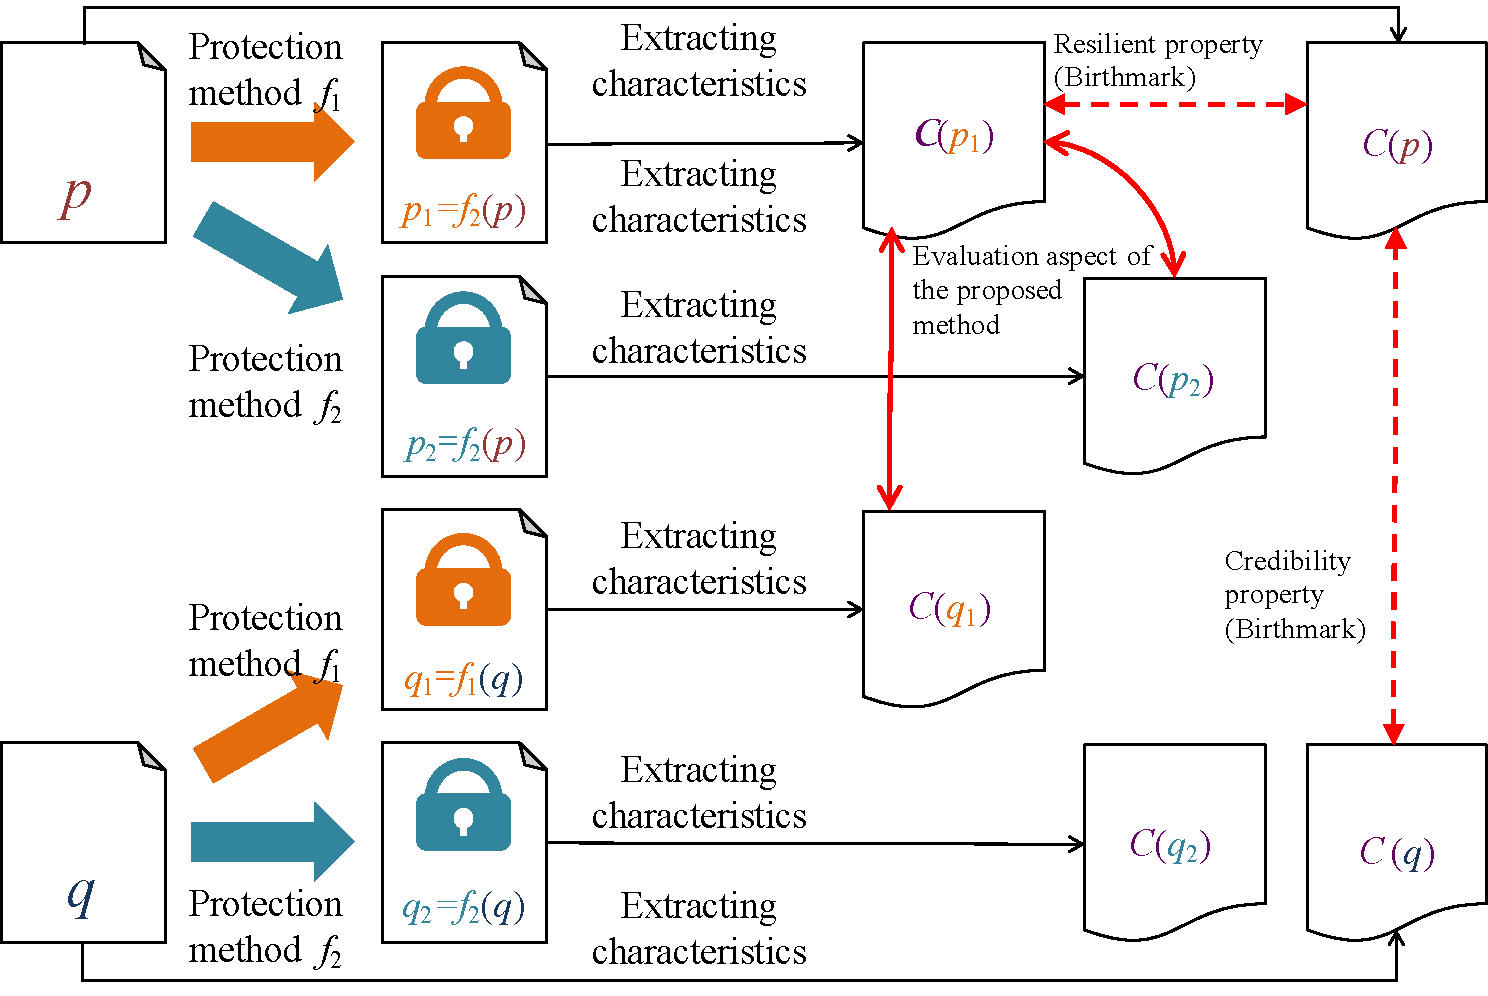
\includegraphics[width=0.78\textwidth]{images/key_idea}
  \caption{提案手法の模式図}\label{fig:keyidea}
\end{figure}


Base mark that is to distinguish others programs by characteristic in program is proposed\cite{tamada05ieice}.
Base mark is technique that is to find plagiarism by comparing characteristic with ones that program have originally.
For difference purpose from this research, it can not apply the base mark as it is, but it can expect the advance method of base mark as standard way of comparison.

Kanzaki's propose method that is to evaluate unnatural of program\cite{kanzaki14ipsj}.
This program is to expect n-gram from opcode in program and to evaluate unnatural by requiring generative probability.
For example, Matuda's evaluate difficult discovery of method of protection by comparing unnatural of fragment of code\cite{matsuda15ipsj}.

We assume that method of protection have a proper characteristic by forcing on this method.
Thus, for proper characteristic, we try to identify how method of protection are used.
If method of protection can be identified, specializing method of attack for  and attack for the method of protection understanding to method of protection are possible.
Conversely, if method of protection can not be identified, the key of attack can not be taken  and attack is difficult.

It show a schematic diagram of method of protection at Figure\ref{fig:keyidea}.
Process method and base mark are same as processing that is to extract characteristic from protected program.
On the other hand, evaluation point are different.
%式が出るので後
In Figure\ref{fig:keyidea}, protected program $p_1=f_1(p)$,
$p_2=f_2(p)$ are gotten by any methods of protection $f_1$ と $f_2$ with program $p$.

So, any characteristics $\birth{p_1}, \birth{p_1}, and \birth{p_2}$ are gotten from $p,
p_1, p_2$ , for using the feature extraction function$\mathcal{C}$.

The interest in base mark technology is part of showing a arrow by a dotted line in Figure\ref{fig:keyidea}.
As a result, we evaluate that how do $\birth{p}$, $\birth{p_1}, and \birth{p_2}$ look like?, and how do $\birth{p}$ and $\birth{q}$ look difference?


The interest in proposed method is part of showing a arrow by a solid line in Figure\ref{fig:keyidea}.
That is to say, we compare that how do protected same programs by different method look difference ($\birth{p_1}$と$\birth{p_2}$)? and how do protected different programs by same method look like?  


\subsection{Characteristic extraction method}
Although Extracting characteristic is like base mark in method,
it do not carry out as expected to itself.
%式が出るので後

Because, in protected different program $p$ and $q$ by same method $f_1$, as base mark is that program itself is to difference, we expect result as difference($\birth{p_1} \neq\birth{q_1}$).
However, as proposed method is to take the characteristic in method of protection itself, we expect result as same($\birth{p_1} \approx \birth{q_1}$).

Therefor, we observe Kanzaki's propose method that is to evaluate unnatural of program\cite{kanzaki14ipsj}

This method is to use the rare in $n$-gram of opcode.
In method of protection, the case is absolutely to insert the sequence of orders in place that is not carried out impossibility, and other case is to rearrange rare order as understanding in original order is difficult.

Thus, we can judgment whether rare order is true or false as showing rarity.
it is to say that these rare order is characteristic in method of protection.
creation probability use the perplexity\cite{gekka14scis}.
Perplexity is known average branch and ais index that express complexity as language.
It is express that the more little this value is,the more next coming language is predicted.
As a result, it is say that the more little the value is, the more natural value is.

On the other hand, in the method of protection, the case is that the compiler outputted original orders with repeated.

As The original order is difference with use frequency, it is not to say the rare.
Thus, the only creation probability is not able to observe the characteristic in method of protection.
Therefor, we observe the frequency in $n$-gram.

In the above, we extract order in $n$-gram from program, and are characteristic in method of protection with the rare ( perplexity ) and frequency.
%

\subsection{Indication of characteristic}
In the proposed method, we measure the characteristic of method of protection how n-gram of opcode before and after in method of protection were changed.
Thus, we measure four indications how n-gram was changed.

%%
First, as taken program is $p$, $p_a$ is protected program $p$ by method of protection $f_a$
($p_a=f_a(p)$).
And, as collective in $n$-gram that extracted from $\mathcal{N}_n(p)$ to $p$, $\distinct{p}$ is collective that removed after repeated n-gram.
And, $\bm{p_a}=\{ (k^a_1, v^a_1), (k^a_2, v^a_2), ..., (k^a_m, v^a_m) \}$ is frequency vector 
of $\mathcal{N}_n(p)$.
At this time, when program is gotten to converse $p$ to $p_a$, we measure the characteristic in method of protection with next four index. 

\begin{enumerate}
\item 追加された$n$-gramの数 $M_a=$($\overline{\distinct{p}} \cap \distinct{p_a}$)、
\item 削除された$n$-gramの数 $M_d=$($\distinct{p} \cap \overline{\distinct{p_a}}$)、
\item $\distinct{p}$と$\distinct{p_a}$のJaccard係数 $M_j=$($\displaystyle
  \frac{|\distinct{p} \cap \distinct{p_a}|}{|\distinct{p} \cup
    \distinct{p_a}|}$)、
\item $\bm{p}$と$\bm{p_a}$のコサイン類似度 $M_c=$($\displaystyle
  \frac{\sum_{i=1}^{m} v_i v^a_i}{\sqrt{\sum_{i=1}^m v_i}
    \sqrt{\sum_{i=1}^m v^a_i}}$)
\end{enumerate}
%

This is a considerable with similarity calculation in method of base mark.
However, the observed point in this method is $p$と$p_1$ or $p_1$と$q_1$.
Thus, we do not observe a comparison of general same program, 
for example, $p$ and $q$ as base mark.



%式が出るので後

%%%前回の予備実験のセクション
%\section{preliminary experiment}
%\subsection{summary}
%Before performing the evaluation experiment, we carry out preliminary experiment.
%
%This purpose is confirmation that is to detect appearing characteristic in method of protection by proposed method.
%Therefore, it obfuscate jar file p,q,r in really for using the obfuscation tool as target to Java.
%
%%式が出るので後
%This method of obfuscation is correspond to fn
%
%
%\subsection{Comparison by the proposed indication}
%
%
%\subsection{histogram in n-gram of opcode}
%
%\subsection{perplexity in n-gram of opcode}
%
%\subsection{analysis in extracted n-gram}


\section{Experimental evaluation}
\subsection{Overview}


そこで、Javaを対象とした難読化ツールを用い
て、実際にjarファイル$p, q, r$を難読化する。この難読化手法が$f_n$に相
当する。そして、難読化前後のjarファイルから特徴$\birth{p}, \birth{q},
\birth{r}, ..., \birth{p_n}, \birth{q_n}, \birth{r_n}$を抽出する。そし
て、得られた特徴をグラフにして、互いに比較する。

抽出する特徴は、第\ref{sect:artificiality}節で述べたようにオペコードの
$n$-gramを基本とし、そのパープレキシティと頻度を用いて比較を行う。

パープレキシティを導出するためにコーパスの構築が必要である。そのため、
The Apache Software Foundation\footnote{\url{http://www.apache.org/}}
で配布されているjarファイル 3,786 個を収集した。jarファイル内の総クラ
ス数は 660,465、総メソッド数は 4,272,567 である。

Some characteristic in method of protection have become clear by preliminary experiment.
This purpose is how to decide the method of protection from extracted characteristic.
As extracting characteristic is based on n-gram of opcode such as 
chapter three, verse 2, 
we compare its with perplexity and frequency.

we conducted a preliminary study to investigate the following questions.
RQ1: What kind of characteristic in method of obfuscation? 

RQ2-1:Is the characteristic effective measure for unknown product?

RQ2-2:Is the characteristic effective measure for unknown obfuscation?

\begin{table}[t]
  \centering
  \footnotesize{
    \caption{利用したJarファイル一覧}\label{table:jars}
  \begin{tabular}{l|r||l|r||l|r}
    Product & Version & Product & Version & Products & Version \\ \hline
    ASM       & 3.3.1 & FakeHack  & 1.0 &JCalendar & 1.3.3   \\
    Jhstop    & 0.0.1 & Jwhich    & 1.0   & Robocode-setup & 1.6.0.1 
  \end{tabular}
  \caption{利用した難読化ツール}\label{table:tools}
  \begin{tabular}{ll|l}
      Tools & Abbr. & Overview \\ \hline
      Allatori Java Obfuscator & ALL & 商用の難読化ツール \\ \hline
      ProGurad                 & PG & OSSの難読化ツール \\ \hline
      Sandmark                 & & 研究用の難読化ツール \\
      \hspace{0.2cm} Duplication registers & DR & 代入を重複させる。\\
      \hspace{0.2cm} Merge local integers & MLI & 2つのint変数をlongに収める。\\
      \hspace{0.2cm} Irreducibility       & IRR & 制御フローを複雑にする。\\
  \end{tabular}}
\end{table}

\subsection{analysis in n-gram}
In this purpose, we analyzed order in n-gram by referring to frequency and perplexity in each method of obfuscation.
In the analysis result, It see different order before and after protection in method of obfuscation.

As a result, we analyze the RQ1.

Also, we understand that added order is high value of perplexity and rare order.
For these data, added order
As characteristic in method of obfuscation is added order by these datas, the characteristic are reported TABLE\ref{table:features}.



\begin{table}[t]
  \centering
  \footnotesize{
    \caption{ツールごとの特徴}\label{table:features}
  \begin{tabular}{l|l}
    ツール              & 特徴 \\ \hline
    ALL & オリジナルの命令列を\texttt{swap}命令で入れ替える \\
    PG  & オリジナルと変化なし \\
    DR  & \texttt{istore}命令を2回続けて実行する \\
    MLI & \texttt{dup2x2 lxor}を連続して実行する \\
    IRR & \texttt{nop}命令がある \\
  \end{tabular}}
\end{table}


\subsection{identifying method of obfuscation in known}
In this purpose, unknown product are obfuscated by using the tools in TABLE\ref{table:features}, after we identify how method of obfuscation are used.

As a result, we analyze the RQ2-1.

Not appearing n-gram are researched by n-gram that is before applied obfuscation.
In the result, n-gram of high frequency in five is reported TABLE\ref{table:junit}.
In showing the TABLE\ref{table:junit}, the order are called high value in perplexity such as dup2X2 lxor.
As the order is characteristic, we compare it with characteristic in five tool ( TABLE\ref{table:junit} ).
As a result, characteristic in applied method of obfuscation correspond with characteristic in method of MLI.

\begin{table}[t]
  \centering
  \footnotesize{
    \caption{JUnit (5-gram)の命令列}\label{table:junit}
  \begin{tabular}{l|r|r}
    命令列 & 頻度 & PPL\\ \hline
 %   \multicolumn{1}{p{1cm}}{ORI} & 
 %   \multicolumn{1}{p{1cm}}{ALL} & 
 %   \multicolumn{1}{p{1cm}}{DR} & 
 %   \multicolumn{1}{p{1cm}}{IRR} & 
 %   \multicolumn{1}{p{1cm}}{MLI} & 
 %   \multicolumn{1}{p{1cm}}{PG} & 
 %   \multicolumn{1}{p{1cm}}{PPL} \\ \hline
    \texttt{dup2x2 lxor lconst\_1 lneg bipush}   & 16 & 11.30E+05 \\
    \texttt{lload dup2x2 lxor lconst\_1 lneg}    & 16 &   5.37E+05 \\
    \texttt{bipush lushr land lxor lstore}       &  9 &   0.52E+05 \\
    \texttt{lconst\_1 leng bipush lushr land}    &  9 &   0.96E+05 \\
    \texttt{lneg bipush lushr land lxor}         &  9 &  1.37E+05 \\
  \end{tabular}}
\end{table}

\subsection{identifying method of obfuscation in unknown}
In this purpose, known products are obfuscated by using the unknown method of obfuscation, after we identify how method of obfuscation are used.

As a result, we analyze the RQ2-2.

Not appearing n-gram are researched by n-gram that is before applied obfuscation.
In the result, n-gram of high frequency in five is reported TABLE\ref{table:jhstop}.
In showing the TABLE\ref{table:jhstop}, the order that is high value in perplexity are called dup and imul orders in continuous.
As the order is characteristic, we compare it with characteristic in five tool ( TABLE\ref{table:jhstop} ).
As a result, characteristic in unknown method of obfuscation do not correspond with characteristic in analyzed method.

In the next, as difference product are obfuscated unknown method of obfuscation, we compare the each characteristic.
As a result, as the same characteristic are identified, we understand that unknown method of product is method of SOP.


\begin{table}[t]
  \centering
  \footnotesize{
    \caption{Jhstop (5-gram)の命令列}\label{table:jhstop}
  \begin{tabular}{l|r|r}
   命令列 & 頻度 & PPL\\ \hline
 %   \multicolumn{1}{p{1cm}}{ORI} & 
 %   \multicolumn{1}{p{1cm}}{ALL} & 
 %   \multicolumn{1}{p{1cm}}{DR} & 
 %   \multicolumn{1}{p{1cm}}{IRR} & 
 %   \multicolumn{1}{p{1cm}}{MLI} & 
 %   \multicolumn{1}{p{1cm}}{PG} & 
 %   \multicolumn{1}{p{1cm}}{PPL} \\ \hline  
    \texttt{irem iconst\_0 if\_icmpne aload getfield} & 15 &   0.15E+05 \\
    \texttt{dup dup dup imul imul}                    & 14 &  42.40E+05 \\
    \texttt{dup dup imul imul isub}                   & 14 &   8.74E+05 \\
    \texttt{dup imul imul isub iconst\_3}             & 14 &   3.49E+05 \\
    \texttt{iload dup dup dup imul}                   & 14 & 101.00E+05 \\
    \end{tabular}}
\end{table}


\section{Conclusion}
In this paper, we took the identification of method of protection by watching the unnatural evaluation.
The actual program was applied method of protection and extracted characteristic to base on frequency and perplexity to order line of n-gram.
In this evaluation experiment, the identification of known obfuscation is easy and the identification of unknown obfuscation is difficult.
This solution plan is to increase the characteristic of method of obfuscation.
it can respond to method of unknown obfuscation by increasing characteristic. 


% conference papers do not normally have an appendix


% use section* for acknowledgment
\section*{Acknowledgment}


% trigger a \newpage just before the given reference
% number - used to balance the columns on the last page
% adjust value as needed - may need to be readjusted if
% the document is modified later
%\IEEEtriggeratref{8}
% The "triggered" command can be changed if desired:
%\IEEEtriggercmd{\enlargethispage{-5in}}

% references section

% can use a bibliography generated by BibTeX as a .bbl file
% BibTeX documentation can be easily obtained at:
% http://mirror.ctan.org/biblio/bibtex/contrib/doc/
% The IEEEtran BibTeX style support page is at:
% http://www.michaelshell.org/tex/ieeetran/bibtex/
\bibliographystyle{IEEEtran}
% argument is your BibTeX string definitions and bibliography database(s)
\bibliography{sagisaka}
%
% <OR> manually copy in the resultant .bbl file
% set second argument of \begin to the number of references
% (used to reserve space for the reference number labels box)
%\begin{thebibliography}{1}
%
%\bibitem{IEEEhowto:kopka}
%H.~Kopka and P.~W. Daly, \emph{A Guide to \LaTeX}, 3rd~ed.\hskip 1em plus
%  0.5em minus 0.4em\relax Harlow, England: Addison-Wesley, 1999.
%
%\end{thebibliography}




% that's all folks
\end{document}


